\chapter{Background}\label{Background}

\section{Renal cell carcinoma}

Renal cell carcinoma (RCC) is a heterogeneous collection of tumours that originate from renal tubular epithelial cells. During the past 20 years, significant developments in the histopathological and molecular characterisation of RCC have resulted in substantial adjustments in its classification. Clear cell RCC (ccRCC), papillary RCC (pRCC), and chromophore RCC (chRCC) are the main subtypes with incidences greater than or equal to 5\%. If a tumour does not match any of the subtypes of diagnostic criteria, it is referred to as unclassified RCC (uRCC). \cite{Hsieh2017Renal} 
With Approximately 75\%, ccRCC is the most prevalent subtype and also accounts for the majority of deaths from kidney cancer. \cite{Hsieh2017Renal} Once ccRCC develops metastases, survival chances are poor, with a median survival of 13 months and only 10\% of patients survive for more than 5 years. \cite{Cohen2005Renal}
That being said, the classification of subtypes is not always simple, since pRCC and chRCC can also show the presence of clear cells, so around 4\% of cases have to be classified as uRCC. \cite{Hsieh2017Renal, LopezBeltran20062004}
Treatment of localised RCC involves partial or complete removal of the organ (nephrectomy), destruction of the tissue using extreme temperatures, either hot or cold (ablation) or active surveillance using radiographic methods. Despite these attempts, around 30\% of patients with ccRCC eventually develop metastases. Therapies that target specific pathways exist, but do not stop cancer progression entirely. In addition, the effectiveness of the treatment varies from patient to patient. Immunotherapy is another treatment approach, but has fallen out of favour in recent years; because commonly used drugs show high levels of toxicity while only being successful for a small subset of patients. New drugs targeting a variety of proteins are still being investigated. Another issue are resistances to single drugs that make multi-agent treatments necessary. \cite{Hsieh2017Renal}

The main risk factors for RCC include excess body weight, hypertension, and smoking; others are chronic kidney disease, hemodialysis, a kidney transplant, acquired kidney cystic disease, and diabetes mellitus.
Not all characteristics of the RCC cell can be studied in cell lines \textit{in vitro}. Hence, it is even more important to find new ways to conduct research on samples \textit{in situ}, such as tissue samples.
Mutations in the following genes have been linked to RCC: BAP1, FLCN, FH, MET, PTEN, SDHB, SDHC, SDHD, TSC1, TSC2 and VHL. While, other genes are suspected as well, the evidence is not as clear. \cite{Hsieh2017Renal}
More recently, the Von Hippel–Lindau (VHL) gene and the protein polybromo-1 (PBRM-1) gene have been identified to show genetic mutations in RCC. The former is a tumour suppressor gene that regulates the concentration of intracellular proteins and hypoxia-inducible factor 1 alpha and 2 alpha. A defect has been shown to result in upregulation of mRNA encoding for growth factors. \cite{Padala2022Clear}


\section{Histopathology}

\subsection{Different kinds of tissue}

Human tissue is classified into four basic tissues. 
The first is the epithelium. The epithelial cells form glandular tissue and lines the lumen of organs and body cavities. It also covers externals of the organs. The same is true for the human body itself, as the epidermis consists mostly of these cells. Therefore, epithelial cells have a bipolar structure, where basal refers to the inward oriented and apical to the outward oriented sides of the cell. Other epithelial cells densely cover the remaining sides. 
As there is no space for blood vessels in between the layer of epithelial cells, they are exclusively supplied with nutrients and oxygen from the basal side. The epithelium is further subdivided into types based on the characteristics of their layers, the shape of the cells, and their functional specialisations. The epithelium layers are called simple if there is only one layer that covers the tissue. In the case that there are multiple layers but only the innermost is in contact with the basal membrane, they are referred to as stratified. Each cell is either described as squamous, where the cell volume is small and the size of the nucleus is responsible for the phenotype. Cuboidal cells have round nuclei that are centrally located, while the cells themselves appear squared with relatively equally long sides. Columnar cells have a basally located nucleus and are relatively thin in appearance. Epithelial cells can have cilia to move particles; microvilli, to increase the surface area; and keratin, to enhance the structural stability of the tissue. 
The various combinations of these characteristics define the different functional types of epithelial cells.

The next type is connective tissue, of which 4 types exist and all derive from the same embryonic tissue called mesenchyme. All types are made up by a small number of cells which is surrounded by an extracellular matrix. Unlike epithelial cells, there is much space between these cells. One type is proper connective tissue, including fat-storing adipocytes and macrophages, which degrade microorganisms or damaged tissue. The cell types are further classified by the density and regularity of the cells and their extracellular matrices. 
Another type of connective tissue is cartilage, whose subtypes are found in very specific organs or body parts. Generally, the tissue is very durable while still very flexible. Thus, it can absorb shock very well.

Bone tissue is the third type of connective tissue. It is controlled by osteocells, which are responsible for the creation, maintenance, and breakdown of the bone matrix.
The last type is blood, which is made up of erythrocytes, leukocytes, and thrombocytes to handle oxygen transport, immune defence, and blood clotting, respectively.
The third type of tissue is muscle tissue, which is either skeletal or cardiac. The former is also organised into muscle fibres, of which multiples make up a muscle fascicle. Multiple fascicles then make up a skeletal muscle. Each of these substructures is compartmentalised by connective tissue. The tissue of this structure is attached to the bones.

Cardiovascular muscle tissue is found exclusively in the wall of the heart. It only differs from smooth muscle tissue in the structural arrangement of myosin and actin molecules. This third type makes up hollow organs such as arteries or the stomach.
Lastly, there is nervous tissue, which is split into neurons and neuroglial cells. Neurons are the central cells of the nervous system. They transport information internally \textit{via} electric action potentials and between neurons \textit{via} neurotransmitters that one neuron secretes and the other detects \textit{via} receptor proteins. Neuroglia are the cells that support neurons, both physically and metabolically. \cite{Ash2017Authors}

According to the above, kidney tissue does not contain a single type, but a complex mixture of tissue types and their respective subtypes. Hence, we can observe various different arrangements within the renal tissue, adding to the complexity at the supracellular level. This undermines the need for modern methods to better deal with these complexities.

\subsection{From Tissue to slide}

The procedure of tissue extraction is called a biopsy. There are different types of biopsies, some of which are more suitable for the extraction of kidney tissue than others. Percutaneous renal biopsy is the current standard procedure, which is used in over 90\% of cases. During this operation, a needle is inserted into the patient, through which the tissue will be extracted. Using a guidance system, most commonly based on ultrasonic sound (US) or computed tomography (CT). Although both have comparable success rates, CT offers better visualisation, but takes more time and is more expensive.
The only reason why this procedure is not used, is when it is inadequate for one or multiple reasons respective to the condition of the patient. An example of such a reason is morbid obesity. These alternatives involve surgical techniques or different types of needles. \cite{Zhuo2017Alternative}
The other possibility for acquiring tissue samples is nephrectomy. This operation refers to the removal of a kidney and is therefore always surgical. It is performed as part of a kidney transplant or as part of cancer treatment when there is no other option than to remove the affected organ.
\cite{Herr2008Surgical}

\subsection{Differently stained WSIs}

As noted above, there are more images than patients. Hence, there are five images available per patient. However, they differ in the type of stain each slide was treated with. The first batch of images is stained with Haematoxylin and Eosin (H\&E). This combination of chemicals allows for the visualisation of almost all cell components in tissue. Haematoxylin stains nuclei purple, while Eosin stains proteins pink. This allows researchers to easily detect details that would otherwise be difficult or impossible to spot. All other stains use different types of immunostaining, which is based on interactions between antibodies and their antigens. For this reason, such stains can target very specific proteins directly. Because of this specificity, researchers can easily separate proteins of interest from the rest of the image. The first of these stains targets the Cluster of Differentiation (CD) protein 68. CD68 is highly expressed in macrophages and other mononuclear phagocytes. Hence, this protein can be used to detect tumour regions or inflamed tissue areas. It is also used as a predictive marker of patient survival. Within the cell, it is predominantly located in the lysosomal and endosomal compartments. 
CD68 has also been shown to bind to other molecules such as phosphatidylserine or apoptotic cells, and it also serves as a receptor for malaria. \cite{Chistiakov2017CD68/macrosialin}
The next set of slides was stained for CD204 or Macrophage scavenger receptor 1 (MSR1) or Scavenger receptor A (SR-A). This protein plays a role in many metabolic processes, including lipid metabolism and atherogenesis. Furthermore, CD204 is involved in inflammation, innate immunity, host defence, Alzheimer’s disease, virus recognition and uptake, bone metabolism, pulmonary injury, sepsis, cardiac and cerebral injuries. \cite{Kelley2014Scavenger} More interestingly, it also has been shown to induce tumour cell death in prostate cancer cases. \cite{Yu2006CSR1, Zhu2008CSR1}
CD8 and CD20 positive cells were stained together on a single slide. CD8 is a marker that is commonly used to detect T cells. These CD8\textsuperscript{+} T cells are also known as cytotoxic T cells. These cells are an essential part of the adaptive immune response. Although active during all types of infection, they also play a role in the anticancer immune response by identifying cancerous cells as foreign and thus eradicating them. \cite{Raskov2020Cytotoxic, Oh2021Cytotoxic} CD20 is a marker gene for B-lymphocytes. These subtypes of white blood cells produce antibodies that can bind to cancer cells and help to eliminate them. \cite{Murphy2011Janeways} 
The last set of slides was stained for the detection of CD4 and FoxP3. CD4 is a marker for another type of T cell. They also have the ability to kill cancer cells themselves. Hence, they are also found near those cancer cells in human tissue. \cite{Oh2021Cytotoxic} Lastly, FoxP3 has been shown to be correlated with unfavourable prognosis in cancer patients of various types. \cite{Yang2017FOXP3} This is because FoxP3 acts as a suppressor of the anti-tumour immune response. Hence, the possibility to target FoxP3-expressing cells to induce an immune response against cancer is being investigated. \cite{Tanaka2016Regulatory}

\section{Survival Analysis and Loss function}
Survival analysis is a type of regression problem with the notable difference that parts of the training data are censored. 

\subsection{Censored Data}
Since digital pathology usually deals with human patients as sources of data rather than model organisms, censoring of patients is a common occurrence. There are three scenarios under which patients are censored. First, the patient does not experience the event of interest before the study period ends. Next, patients are censored if they fail to attend a follow-up appointment because their status with respect to the study is unknown. Lastly, a patient cannot continue the study for reasons that are not related to the event of interest.
The cases listed above all result in so-called right-censored data samples. The status of these cases can only be observed up to the respective time points of censoring. Methods of survival analysis are adapted to incorporate censored 
data as good as possible. \cite{Kleinbaum2012Cox}

Left-censoring refers to the situation where the exact time of first occurrence of the condition of interest is unknown. The patients are only known to be unaffected at the start of the study, hence the event has occurred some time after the most recent follow up. \cite{Kleinbaum2012Cox} This is rarely the case in biomedicine, as patients are usually already affected when selected for such a study.

\subsection{Survival Analysis}
Survival analysis is a statistical tool in which an outcome of interest is the time passed until an event of interest occurs. Survival analysis typically involves estimating the survival function, which is the probability of survival beyond a certain time point \(t\). This function is represented as \(S(t)\) and can be estimated using various methods such as the Kaplan-Meier estimator, a Weibull distribution or the Cox proportional hazards model. The survival function is given by

\[ S(t) = P(T>t) \]

where $T$ is the time until the event of interest occurs. This is usually modelled using a hazard function \(h(t)\), which denotes a probability of experiencing the event of interest at a time \(t\), given that the individual has not experienced the event up to that point.

% \[ h(t) = \lim_{\Delta t \to 0} \frac{P(t \leq T < t+\Delta t| T\geq t)}{\Delta t} \ge 0 \]
\[ h(t) = \lim_{\Delta t \to 0} \frac{P(T < t+\Delta t| T\geq t)}{\Delta t} \ge 0 \]

The presented formula uses small-time intervals $[t; t+\delta[$, which is a common means of approximation.
Unlike the survival function, which describes the absence of an event, the hazard function provides information on the occurrence of an event.
The relationship between $S(t)$ and $h(t)$ is as follows:

\[ h(t)=-\frac{d}{dt}[logS(t)] \]

Thus, one can easily compute one when knowing the other. \cite{Clark2003Survival}

\subsection{Cox Proportional Hazards Models}
The Cox proportional hazards model is a semi-parametric model that is used commonly for survival analysis. \cite{Cox1972Regression} The model estimates the hazard ratio, which measures the relative risk that the event occurs in one group compared to another, while controlling for other variables. The mathematical expression for the Cox model is as follows:

\[ h(t|X) = h_0(t) \exp(\beta_1 X_1 + \beta_2 X_2 + ... + \beta_p X_{p)}= h_{0(t)} \exp(\beta_{i} X_{i}) \]

 \(h(t|X)\) is the conditional hazard function at time \(t\) for an individual with covariate values \(X = (X_1, X_2, ..., X_p)\), and their regression coefficients \(\beta = (\beta_{1}, \beta_{2}, ..., \beta_{p}\)). The exponential function is used to ensure that the hazard ratio stays greater than or equal to zero. \(h_0(t)\) is the baseline hazard function that is common to all individuals.

The Cox model assumes that the hazard rate is proportional across different levels of the covariates. The proportional hazards assumption can be formulated as:
\[ \frac{h(t|X)}{h(t|X')} = \exp(\beta_1 (X_1 - X'_1) + \beta_2 (X_2 - X'_2) + ... + \beta_p (X_p - X'_p)) \]
where $X'$ is the vector of covariates for the reference group. Note that the baseline hazard was cancelled. This in turn means, that the ratio of hazards of two subjects is constant and independent of time.
Furthermore, the model is linear, and thus assumes a linear increase or decrease of a patient's risk over time. It is self-explanatory that this a strong generalization and can end up being a bad approximation of the true relationship. \cite{Deo2021Survival} However, DNNs manage to lift this restriction, by introducing non-linearities \textit{via} their architecture.

\subsection{Derived Loss Function}
The Cox Proportional Hazards (CPH) likelihood function can be written as follows:

\[ L(g) = \prod_{i|\delta_{i}=1}^{n}\frac{\text{exp}(g(x_i))}{\sum_{j|t_{j}\ge{t_{i}}}\text{exp}(g(x_j))} \]

where $n_i$ is the current observation out of a total of $n$ observations. The event indicator $\delta_i$ represents the outcome of the observed event. The event occurred within the time of the study if $\delta_i=1$ and \(0\) otherwise. We refer to the latter observations as censored. Hence, the numerator consists only of sampled from the uncensored subset of observations. The denominator represents all observations $j$ with a survival time $t_j$ higher than that of the current $t_i$. In other words, these individuals are still at risk for the event to occur. Thus, the numerator represents the relative hazard of the current individual.
$g(x_i)$ represent the non-linear output of the neural network, and thus the coefficients \(\beta\) applied to the input \(X\).
From this, the negative log likelihood is derived as the loss function to be minimized as

\[ LL(g) = \sum_{i|\delta_{i}=1} \text{log} \left(\sum_{j|t_{j}\ge{t_{i}}} \text{exp} (g(x_{j})) \right)- g(x_{i})\]

Tied event times can be handled using the Breslow approximation method, which assumes that individuals with tied event times were selected from the same risk set. Those observations simply share the same denominator in the CPH likelihood. \cite{Breslow1974Covariance, Yang2022FastCPH}

\subsection{Concordance index}
The concordance index (C-index) is a commonly used metric for measuring the performance of survival forecasting methods. This function does consider uncensored cases in its computation. If the event for sample $j$ occurred before the time of censoring of sample $i$, we can still include them in one-sided fashion.  \cite{Schneider2022Integration}
The C-index is computed as follows: 
\[  C = \frac{\sum_{i,j:t_{j}<t_{i}} 1_{g(x_{j}) > g(x_{i})}\delta_{j}}{\sum_{i,j:t_{j}<t_{i}} \delta_{j}} \]
where $i$ and $j$ are samples that are being compared, $t$ denotes their respective survival times and $\delta$ their censoring status ($\delta = 1$ if uncensored, else $0$). The network is denoted by $g$ and the sample is denoted by $x$.\cite{Yang2022FastCPH} Thus the c-index ranges from zero to one, the higher the value, the better the predictions. That being said, it is important to note that this metric only measures concordance. Because of that, the actual distance between predicted risk and true survival time is not relevant. The C-Index is only concerned with \textit{which} patient lives longer and not \textit{how much} longer.

\begin{figure}[h!t]
     \centering
     \begin{subfigure}[b]{0.49\textwidth}
         \centering
         \includegraphics[width=\textwidth]{latex/figures/C-Index_uncensored.png}
         \caption{only uncensored samples}
         \label{fig:uncensored}
     \end{subfigure}
     \hfill
     \begin{subfigure}[b]{0.49\textwidth}
         \centering
         \includegraphics[width=\textwidth]{latex/figures/C-Index_censored_noz.png}
         \caption{censored and uncensored samples}
         \label{fig:censored}
     \end{subfigure}
     \caption[Concordance Index Diagram]{Illustration of pairwise relationships for concordance index calculation. Square nodes are uncensored, circle nodes are censored. Edges depict whether a directional comparison is made. The illustrations were drawn using the graph visualization software graphviz. \cite{Gansner2000Open}
     }
\end{figure}
As subfigure $a$ only contains uncensored samples, each node is connected to all nodes with higher survival times. For the subfigure \(b\), samples $x$ and $y$ are censored. Hence, there are no outgoing edges from these two samples, as the final outcome is unknown. However, since our model predicts hazards for them too, these nodes can be considered by all uncensored samples with survival times lower than the time to censoring just as they were regular samples. 

\section{Deep learning}

% \subsection{Neurons?}

% While the true similarities are questionable, neural networks are ofthen compared to the structure of the nervous tissue from the previous section...

\subsection{Multimodal deep learning}

Multimodal Deep learning describes any kind of neural network that involves multiple kinds of input data that can be separated from each other by at least one aspect. Modalities can be text, images, audio, or anything different enough to justify an auxiliary process. In the context of digital medicine, the modalities are usually defined by the origin of the data or its method of collection. Therefore, although DNA and RNA sequences can be defined as strings of letters from a small subset of the Latin alphabet, they are considered different modalities due to the underlying biological processes and structure.
This broad definition of multimodal fusion includes many methods. A field of multimodal methods that gained widespread popularity over recent years are generative models, where one modality is commonly transformed into another. Again, in the context of digital medicine, we are usually interested in combining multiple modalities as input to be processed by the deep neural network. Hence, the main challenge that is specific to multimodal models is the so-called fusion of these modalities.
Multimodal fusion as a technique can be subdivided into three categories. The main difference between them is the time point at which the fusion operation occurs during the forward pass through the model. The following shall give an overview over different approaches that are being employed in digital pathology.

\subsubsection{Early Fusion}

Early fusion associates the input data first, before propagating it through any layers of the neural network. Among other methods, this can be achieved by simple vector concatenation, bilinear pooling, 
\cite{Tenenbaum2000Separating}
an element-wise sum or multiplication. One advantage is its simplicity, since only a single model has to be designed, optimised, and trained. Furthermore, within-modality and cross-modality correlations are learned simultaneously and immediately. This has the effect that even at low levels of abstraction, different modalities can influence one another. For example, when analysing image data, a convolutional neural network (CNN) is usually used to learn higher level structures like shapes of objects. \cite{Stahlschmidt2022Multimodal}
By early fusion with unrelated data, this can get disturbed, leading to worse results overall. Furthermore, the model has to be suitable for each modality, which is rarely the case if they differ substantially. This works especially well if the inputs adhere to some form of synchronisation. For example, when video data is combined with the corresponding audio. \cite{Lipkova2022Artificial}
However, relations at higher levels of abstraction are also more challenging to detect because of this. \cite{Stahlschmidt2022Multimodal}

\subsubsection{Late Fusion}

On the opposite end of the spectrum, there is late fusion. Here, single-modality networks are trained fully independent of each other and each model performs its own predictions. The separate outputs are then aggregated, either by some naive pooling operations or with mechanics that make use of learnable parameters. The latter makes it possible to factor in the different impact that the modalities might have on the task of the network. Examples are averaging\cite{Huang2020Multimodal}, Bayes-based rules \cite{Reda2018Deep}, or majority voting. \cite{Morvant2014Majority}
The advantages of late fusion are that it does not pose constraints on data synchronisation, works with missing data as each model is self-contained and predictions are aggregated. New modalities can be easily added to the new model, and it is not necessary to retrain all submodels. Also, primitive co-variates can easily be included near the end of the pipeline. In contrast, this would require some considerations to be possible with early fusion. 
Overall, this can work well with unbalanced amounts of data, so that a lack of data from one modality cannot negatively impact the others. Also, if no strong interdependencies between modalities are to be expected or when the information density varies significantly between modalities. \cite{Lipkova2022Artificial, Stahlschmidt2022Multimodal}

\subsubsection{Intermediate Fusion}
Intermediate fusion is a more complex method than the two mentioned previously, which is why it only gained popularity more recently. Here, the modalities are fused during the training progress and at different levels of abstraction. This allows the model to learn within-modal correlations first and inter-modal correlations afterwards. Alternatively, separately extracted features can be fused and directly advanced to the prediction.
Lipkova \textit{et al.} further sub-categorises the intermediate fusion process. In the simplest form, all modalities are fused at once. Second, fusion can be performed gradually, where highly correlated channels are prioritised for earlier fusion steps. This forces the network to consider cross-correlations between certain modalities first, and less correlated data is fused only afterwards. This can help increase the performance of the network. Lastly, fusion can be done in a guided manner, where one modality takes a leading role. With the use of co-attention scores, the relevance of the features found in one modality while in the presence of another can be determined. \cite{Lipkova2022Artificial} 
Stahlschmidt \textit{et al.} also define subgroups of intermediate fusion.
First marginal fusion, where features are extracted separately and only fused before entering the fully connected head of the network. Second joint fusion denotes the case when fusion happens during the extraction of features. This allows to learn joint features, that would not be apparent otherwise. However, this approach might also require stronger regularisation. \cite{Stahlschmidt2022Multimodal}
The main advantage of intermediate fusion lies in its flexibility. The depth and approach are aspects that can be tuned to further optimise the performance of the model. Another advantage of intermediate fusion, which it shares with late fusion, is that heterogeneous network design is possible. The feature extraction models can be chosen to best represent their modality. If the modalities differ vastly, this becomes especially important. Nonetheless, intermediate fusion also imposes some restrictions. For once, the size of the output of each sub-model needs to be compatible for the desired fusion method, which limits some networks more than others. \cite{Stahlschmidt2022Multimodal}

Figure \ref{fig:fusion_graphs} illustrates these different approaches. While in early fusion, the fusion happens preliminary to the network processing, it is done in between networks for intermediate fusion. Meanwhile, in late fusion, the predictions of independent networks are combined.

\begin{figure}[h!t]
    \centering
    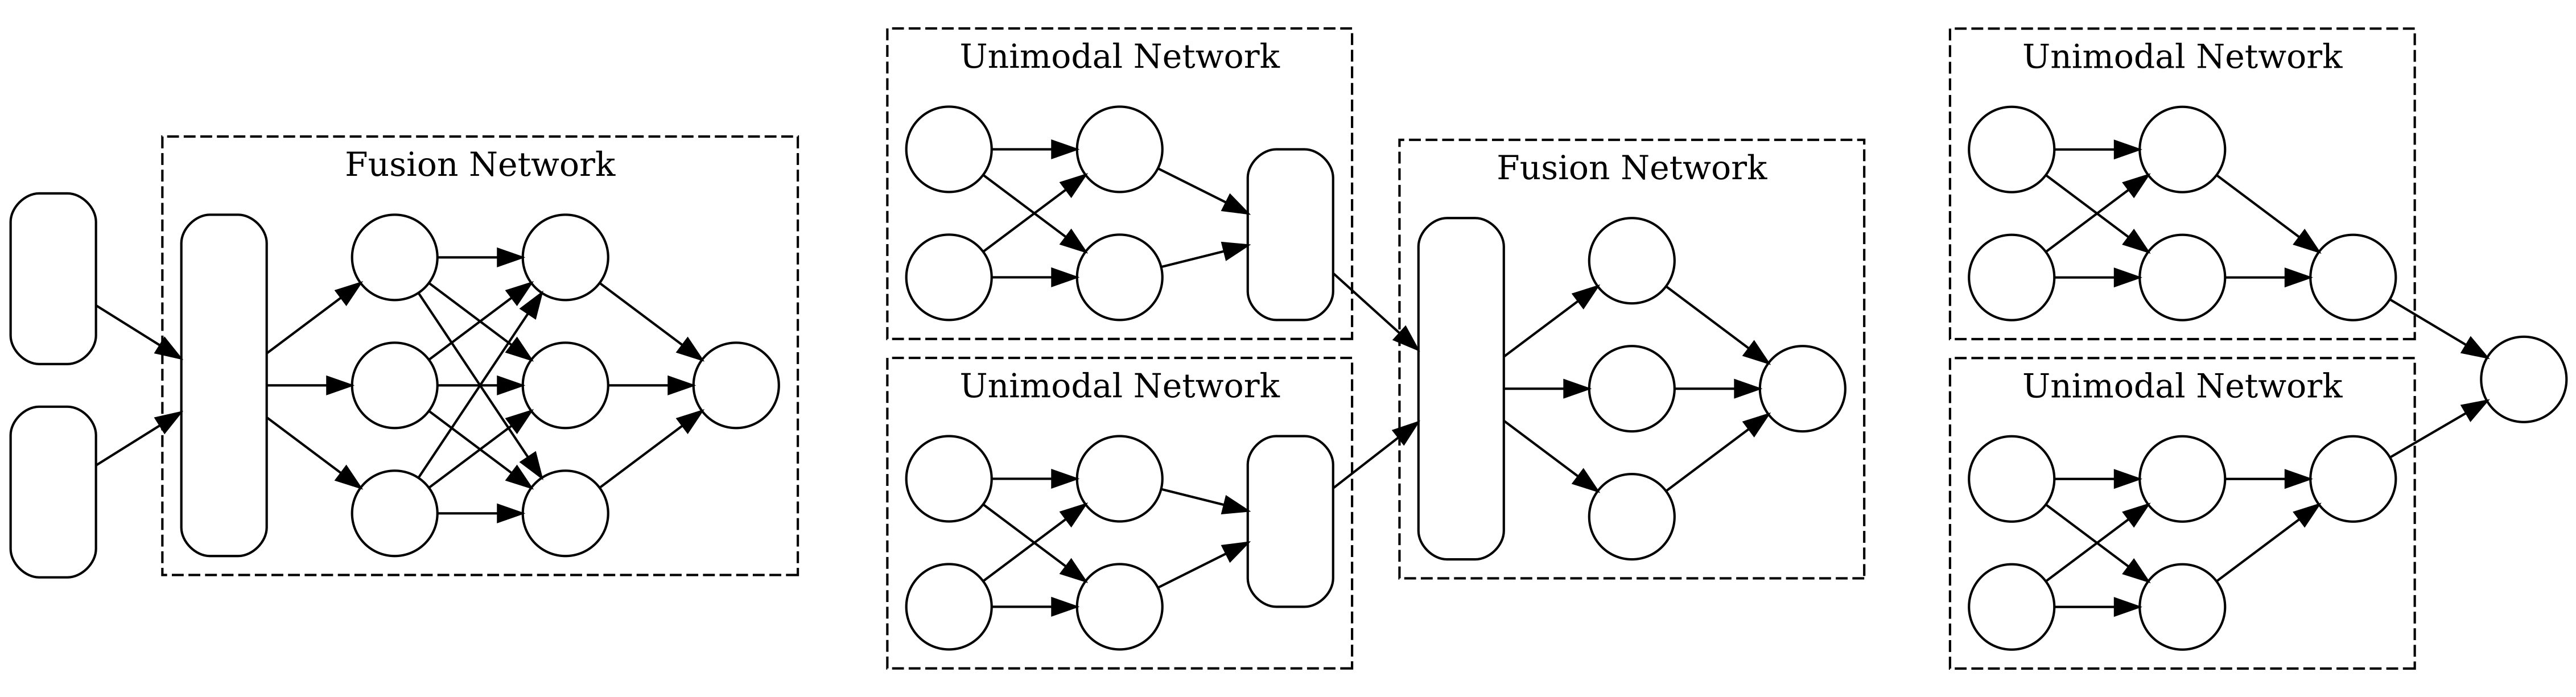
\includegraphics[width=\textwidth]{latex/fusion/all_fusion.png}
    \caption[Multimodal Fusion categories]{Illustration of different variants of fusion networks. Shown on the left is early fusion, intermediate fusion is shown in the middle and late fusion is shown to the right. The illustration was created with graphviz. \cite{Gansner2000Open}}
    \label{fig:fusion_graphs}
\end{figure}


\subsection{Biomarker Detection and Model interpretability}

Model interpretability is an important factor when developing modern deep learning systems, for which there are multiple reasons. By making a model interpretable, it is easier to trust its predictions but also helps to make it more accountable in case of false prediction. These tools help us to understand the prediction, and thus they make it possible to perform targeted changes aiming at improving the model. Another key aspect of interpretability is fairness. By understanding what features of the input the model is attending to, we can detect biases or, in some cases, discrimination with the potential of eliminating these deficits.
As we are interested in biomarker detection, feature attribution methods are most interesting to us. These methods can produce attribution scores for each feature of the input towards the output of the model. Hence, in a WSI, tissue regions of interest could be identified using such tools. For gene expression data, the equivalent would be genes that are especially important for prediction.

\subsubsection{Saliency}

By taking the derivative \(w\) of the image score with respect to the image itself per point in the image, we can obtain a set of weights that attribute the pixels that impact the prediction the most. The Saliency map \(M\) is computed by taking the maximum value of the derivative \(w\)  for each pixel across different channels of the input. This can be denoted as:
\[ M_{ij} = max_c | w_{h(i,j,c)}\]
where \(i\) and \(j\) denote the height and width dimension, and \(c\) the channels of the image. This approach does only require the trained model, a suitable input as well as the obtained score, thus no extra annotations are needed. Furthermore, computation of saliency is cheap as only a single back-propagation pass is performed. \cite{Simonyan2013Deep}
Such a map has the same dimensions as the corresponding input image and can therefore easily be overlaid on top of it.
An extension of saliency maps can be obtained by multiplying the gradient \(w\) by the values of the input, which is inspired by linear models. \cite{Shrikumar2016Not}

\subsubsection{Integrated Gradient}

Integrated Gradients (IG) defines two important axioms that attribution methods should follow to provide good results. The authors note that previous methods such as Saliency \cite{Simonyan2013Deep}, DeepLift \cite{Shrikumar2016Not} or Layer-wise relevance propagation (LRP) \cite{Bach2015Pixel} do not adhere to these axioms.

\paragraph{Defintion: Attribution}

IG defines attribution such that, for a pair of input \(x\) and baseline \(x'\), the attribution \(a_i\) of a single point \(x_i\) is the contribution of that point towards the prediction \(F(x)\). The baseline is needed as a reference point that always produces a neutral prediction. For image tasks, that could be a black image, but is task specific in the end.

\paragraph{Axiom a: Sensitivity}

This axiom demands that, if input and baseline only differ in a single value but still produce different predictions, the corresponding variable should be given a non-zero attribution. Furthermore, the opposite should also be the case. That is, when the alteration of a variable does not change the outcome of a function, it should always have zero attribution.  
Previous methods often fail to ensure this axiom is honored. Because they often rely on Backpropagation, non-linear activation functions, such as ReLU, will impact the process in such a way that this characteristic cannot be fulfilled. \cite{Sundararajan2017Axiomatic}

\paragraph{Axiom b: Implementation Invariance}

This characteristic describes that the attributions for an input should always be the same if the predictions are the same as well. Note that this should be the case for all inputs, i.e. the two networks are considered to be functionally equivalent. This means that this is the case irrespective of the implementation of the network itself, as it is situated between input and prediction (implementation-independence). The authors further use the chain rule as a comparison. \cite{Sundararajan2017Axiomatic} As, this rule states that a derivative can be computed directly or through some intermediaries, knowing the derivative of the intermediary is not essential to the final result. The neural network is compared to such an intermediary by the authors.

\paragraph{Methodology}

Formally, IG is given by the following, with \(\frac{\partial F(x)}{\partial x_i}\) representing the gradient of the neural network \(F(x)\) along the \(i^{th}\) dimension

\[
\text{IG}_i(x) = (x_i - x'_i) \times \int_{\alpha=0}^1 \frac{\partial F(x' + \alpha \times (x - x'))}{\partial x_i} d\alpha
\]

Practically, this can be described as accumulating the gradients between input \(x\) and its baseline \(x'\) along a straight path. Since this is computationally not possible, IG is approximated by summation of a set number of gradients along that path as follows:

\[
\text{IG}_i(x) \approx (x_i - x'_i) \times  \sum_{k=1}^M \frac{\partial F(x' + \frac{k}{M} \times (x - x'))}{\partial x_i} \times \frac{1}{M}
\]

This method can be easily computed, and the number of steps \(M\) defines the granularity of the approximation. As IG only depends on the gradients and not on the network, both axiom a and axiom b hold. \cite{Sundararajan2017Axiomatic}

\subsubsection{GradCAM}

Unlike Saliency Maps and IG, GradCAM is specific to convolutional networks. It assigns attribution values to each neuron for a particular network output with respect to any given convolutional layer of the corresponding CNN. However, usually the last convolutional layer in the network is chosen. 

For this purpose, the feature map activations $f_k(x, y)$ for input \(x\) and score \(y\) with respect to a convolutional layer \(k\) are obtained \textit{via} a single forward pass through the model. The importance weights \(\alpha_k\) of the neurons are then obtained by computation of the gradients \textit{via} backpropagation and combining them with global average pooling as follows

\[
\alpha_k = \overbrace{\frac{1}{Z}\sum_{i=1}^H\sum_{j=1}^W}^{\text{global average pooling}} \underbrace{\frac{\partial y}{\partial f_k(i, j)}}_{\text{gradients}}
\]

where \(Z\) is a normalization constant that ensures \(\sum_k \alpha_k = 1\) and \(H\) and \(W\) are height and width of the input, respectively. The authors describe \(\alpha_k\) as a partial linearisation of the neural network that captures the importance of feature map \(k\). These weights can then be used to obtain a coarse heatmap representing the importance of the inputs to the convolutional layer:

\[
\text{GradCAM}(x) = \text{ReLU}\left(\sum_k \alpha_k f_k(x)\right)
\]

By applying ReLU to the linear combination of weight and feature activation map, we filter for features with a positive influence. Hence, the intensity of these pixels has to be increased to increase the score \(y\). Negative values are likely to result in low attribution. \cite{Selvaraju2016Grad}

Guided GradCAM is a method described in the same publication. It adds the ability to produce fine-grained pixel-space visualisations.
As the matrix obtained from GradCAM has the same dimensions as the input of the considered convolutional layer, it is first upsampled to the dimensions of the input image to allow easy interpretation. The result is multiplied element-wise with the output of guided Backpropagation, another interpretability technique \cite{Springenberg2014Striving}. This fusion of methods produces a high resolution attribution map that determines fine-grained features but also stays discriminative, i.e. it still only attributes to the target task. \cite{Selvaraju2016Grad}

\subsubsection{Occlusion based attribution}

This is a straightforward perturbation based approach that differs fundamentally from the ones presented above. Perturbation methods usually compare the output of the model on the original and on an altered version of the image, to determine the role of the perturbed features. Occlusion based attribution involves replacing a contiguous rectangular region with a given baseline (e.g. an all-zero tensor), and computing the difference in output. \cite{Zeiler2013Visualizing} 

In implementation, this has the effect that the first patched perturbation is applied in the top left corner and then progressed using a sliding window that can produce overlapping regions.Thus, the final patch applied in a direction can be cut-off and thus will be smaller than the  other occlusion patches. The granularity of the attribution map can be defined by the kernel size and the stride. \cite{Zeiler2013Visualizing}

\subsubsection{Attention Mechanisms}

This method is unlike the previous ones, as it is a modification of the network architecture itself and thus learned with each iteration during training.
As we will see later, we use attention mechanisms as a method for feature selection during fusion. However, these methods can also be used for visualising the importance of different inputs. When using a patch-based network, we can apply a simple attention mechanism to determine the relevance of each patch. Thus, we can easily create an attribution map of WSI patches to find regions of high interest. With this technique, the patch size becomes a parameter for the granularity of the biomarker search. \cite{Ilse2018Attention} The advantage of this method is that the attribution of features is computed directly as part of the training process, no extra processing time is needed. However, it also has to be planned for when constructing the network and cannot be just applied as an afterthought, instead full retraining is required if added later to the network. 


\subsection{Neural Network architectures}

This section aims to give a brief overview over the types of neural network used in this work. 

\subsubsection{Residual Networks}

Residual networks are very popular networks for any kind of images analysis task. Originally introduced for classification tasks, they were introduced in 2015 by He \textit{et al.} \cite{He2015Deep} What these networks add to regular CNNs is the concept of a residual block. These blocks usually consist of multiple convolutional layers and their accompanying regularisation techniques (dropout, batch normalisation, etc.). Bypassing such a block is the input that is being processed. It is then added to the output of the block like so \[x_{l+1} = x_l + F(x_l)\] where \(x_l\) is the input to the block and \(F(x)\) is the applied mapping represented by the residual block. This introduces a bias towards the identity matrix of the input, which stabilises gradient propagation that is less impacted by \(F\). \cite{He2015Deep} 
When imagining the network as a space of functions which the network can represent, this allows to narrow down that space by adding complexity but ensures that the new space stays within the previous one at the same time. This way, we can ensure that more complex models will be at least as effective as their predecessor. \cite{Zhang2021Dive}
Another way of looking at it is, that the loss surface becomes much smoother by adding the so-called skip connections than without. \cite{Li2017Visualizing}

\subsubsection{EfficientNet}

The EfficientNet architecture is the result of a Network architecture search (NAS). 
During the search for EfficientNet, network width, network depth, and image resolution were systematically scaled up in a balanced manner. Importantly, the number of floating point operations per second (FLOPS) was directly included into the objective function of the NAS. \cite{Tan2019EfficientNet} This way, the resulting network architecture is supposed to prefer fast training times, hence the name of the network. A previous NAS result, MobileNet, inspired EfficientNet. However, MobileNet was optimized for time of inference or latency. \cite{Howard2017MobileNets, Sandler2018MobileNetV2}
The EfficientNet research shows that bigger input images need more layers to increase the receptive field and need more channels to capture more fine-grained patterns on bigger images. The resulting architecture managed to outperform ResNet on multiple tasks

With the updated version, EfficientNetV2, these results are further improved. By changing the architecture of the residual blocks, they improve the performance of the NAS and of the resulting network further. Originally, the same blocks as in MobileNet were used, and only their parameters were modified. Now, the NAS also looks for a combination between these kinds of blocks.
The authors conclude, that equally scaling up every stage of the network is suboptimal. When scaling up a model, the unequal contributions of layers need to be considered. 
They also argue that increasing the size of the data set is more important than increasing the size of the model in any way. \cite{Tan2021EfficientNetV2} 

\subsubsection{Self Normalising Networks}

These networks improve over regular feed forward or fully connected networks (FNN, FCN). The authors claim that such 
FNNs only perform well if they have a low number of hidden layers. \cite{Klambauer2017Self} This limits the possible level of abstraction and complexity that the networks can represent.
Self-Normalising Networks (SNN) aim to improve upon this by ensuring the following property: each activation maps mean and variance from one layer to the next. Furthermore, outputs stay in the domain of the input, and all points in this domain converge towards a single fixed point. 

\noindent The authors achieve this by combining a scaled exponential linear unit (SeLU) with a new type of layer, which they propose as alpha dropout. The formula for SeLU is given by

\[
\mathrm{SeLU}(x) = \begin{cases}
  \lambda x & \text{if } x > 0, \\
  \lambda \alpha (\exp(x) - 1) & \text{if } x \leq 0,
\end{cases}
\]

\noindent where \(\lambda\) and \(\alpha\) both are scaling factors that help ensure the following conditions required for SNNs

\begin{compactitem}
    \item The presence of negative and positive values are needed to control the mean.
    \item SeLU imposes a lower bound on outputs to dampen the variance.
    \item A slope larger than one to increase the variance if it is too small.
    \item A continuous curve to ensure a fixed point of convergence to exist.
\end{compactitem}

\noindent Alpha dropout is a modification of regular dropout to enable the maintenance of the original mean and variance of the input. Nodes that are selected by the dropout mechanism, get randomized on every forward call, and scaled and shifted to maintain zero mean and unit variance. the authors prove that, with this new regularization scheme, their network outperforms other FNNs with other normalization techniques at a higher number of hidden layers. \cite{Klambauer2017Self}


\subsection{Training Techniques}


\subsubsection{Adam Optimiser}
The Adam optimiser is a gradient-based optimisation algorithm that aims to improve stochastic gradient descent (SGD). The algorithm uses an adaptive learning rate method that is different from traditional SGD algorithms. It maintains exponential moving averages of the gradient and the squared gradient. These are estimations of the first moment (mean) and the second 'raw' moment (non-centred) variance, respectively.

The update rule for the Adam optimiser can be expressed as follows

$$ \theta_t = \theta_{t-1} - \frac{\alpha}{\sqrt{\hat{v}_t}+\epsilon}\hat{m}_t $$

where $\theta_t$ is the parameter vector at time $t$, $\hat{m}_t$ and $\hat{v}_t$ are the bias-corrected first and second moment estimates of the gradient at time $t$, $\alpha$ is the learning rate, $\epsilon$ is a small positive constant used for numerical stability, and $t$ is the iteration number or time. The bias-corrected estimates $\hat{m}_t$ and $\hat{v}_t$ are computed as

\[ \hat{m}_t=\frac{m_t}{1-\beta_1^t},\ \ \ \ \ \ \hat{v}_t=\frac{v_t}{1-\beta_2^t} \]

where $m_t$ and $v_t$ are the first and second moment estimates of the gradient at time $t$, and the hyperparameters $\beta_1$ and $\beta_2$ control the exponential decay rates for the first and second moment estimates, respectively. This bias-correction is necessary due to the initialisation of $\beta_1$ and $\beta_2$ with zero. The raw first and raw second moment estimates are calculated as follows

\[m_t = \beta_1 m_{t-1} + (1 - \beta_1) g_{t}, \ \ \ \ v_t = \beta_2 v_{t-1} + (1 - \beta_2) g_t^2\]

Here, $g_t$ represents the gradient with respect to the objective function at time $t$, and $\beta_1$ and $\beta_2$ are hyperparameters that control the exponential decay rates for the estimates of the first and second moments, respectively. $m_t$ and $v_t$ are both initialised with zero. \cite{Kingma2014Adam} This algorithm is a combination of Root Mean Square Propagation (RMSP) \cite{Hinton2012RMSProp} and AdaGrad. \cite{Duchi2011Adaptive}

AdamW is a modification that adds weight decay to the algorithm. The authors stress that there is a conceptual difference between weight decay and the commonly used $L_2$ regularisation. The authors further argue that weight decay behaves the same as $L_2$ regularisation only if weight decay is coupled to the learning rate, as done in the PyTorch implementation of Adam. Due to dynamic learning rate updates within the Adam algorithm, this can lead to worse generalisation performance than SGD with momentum. as SGD does not suffer from this problem.
AdamW proposes to decouple the weight decay from the gradient-based update. This leads to better generalisation. The authors further note, that AdamW still benefits from a global learning rate schedule. \cite{Loshchilov2017Decoupled}

\subsubsection{Mixed Precision Training}
Mixed precision training is a technique that makes use of smaller data types during the training of a model, which brings two advantages. First, the overall memory requirements are lowered significantly. This enables increased batch sizes, larger models, or larger inputs. More specifically, the inputs and weights are converted to a half-precision data type (float16) before performing the forward pass of the model. The intermediate activations, which are the results of the matrix multiplications and nonlinear activation functions, are also converted to float16 before being passed to the next layer. During the back-propagation of gradients, the gradients are accumulated in single-precision format (float32) to avoid numerical underflow. The accumulated gradients are then converted back to float16 before being used to update the weights of the model. This way, the memory consumption can almost be halved. \cite{Micikevicius2017Mixed}
Second, the training time itself can be reduced. Due to the reduced amount of decimals that need to be approximated, calculations can be done faster. Furthermore, energy requirements are also significantly reduced. \cite{Micikevicius2017Mixed}, \cite{Tagliavini2017Transprecision}
The special \verb|bfloat16| data type was first proposed in 2017 for mixed precision training. This data type preserves the same amount of exponent bits as the IEEE 754 single-precision 32-bit float by solely truncating the mantissa. This stands in contrast to IEEE half-precision 16-bit float, where both exponent and mantissa are truncated, but the mantissa by less fields. This allows the bfloat16 data types to represent the same value range as a regular 32-bit float. \cite{Tagliavini2017Transprecision}
Kalamkar \textit{et al.} were able to show, in 2019, that using this data type achieves the same results as non-mixed precision training. When using the regular 16-bit float, hyperparameter tuning would usually be necessary to achieve this. \cite{Kalamkar2019Study}


\subsubsection{Stochastic Weight Averaging}
Stochastic weight averaging (SWA) is a technique that helps to improve the generalisation of Stochastic Gradient Descent (SGD) and related algorithms.

SWA performs an equal average of the weights traversed by SGD with a modified learning rate schedule. This helps avoid convergence towards the boundary of a minimum. This is especially helpful when the loss surface around the minima resembles a plateau. There, SGD might fail to find a meaningful direction on the gradient. In essence, the weights corresponding to the minimum learning rate per cycle are averaged. \cite{Izmailov2018Averaging}

A variant of SWA is called fast-SWA. After a certain number of training steps within a cycle, the learning rate is adjusted to a lower value. Then, the running average of the weights visited by the optimiser is maintained for the remainder of the cycle and used for further steps. Using this average can be interpreted as simultaneously considering multiple solutions provided by the optimiser; which are the steps since the activation of fast-SWA. since those Solutions lie closer to the boundaries, SWA will help find the centre and thus a better minimum. This has been shown to improve generalisation in computer vision tasks. \cite{Athiwaratkun2018There}
